%% Template for ENG 401 reports
%% by Robin Turner
%% Adapted from the IEEE peer review template

%
% note that the "draftcls" or "draftclsnofoot", not "draft", option
% should be used if it is desired that the figures are to be displayed in
% draft mode.

\documentclass[peerreview,onecolumn]{IEEEtran}
\usepackage{cite} % Tidies up citation numbers.
\usepackage{url} % Provides better formatting of URLs.
\usepackage[utf8]{inputenc} % Allows Turkish characters.
\usepackage{booktabs} % Allows the use of \toprule, \midrule and \bottomrule in tables for horizontal lines
\usepackage{graphicx}
\usepackage{amsfonts}
\usepackage{amsmath}
\usepackage{amssymb}
\usepackage{stackengine}

\usepackage{scrextend}
\changefontsizes{11pt}

\hyphenation{op-tical net-works semi-conduc-tor} % Corrects some bad hyphenation 



\begin{document}
%\begin{titlepage}
% paper title
% can use linebreaks \\ within to get better formatting as desired
\title{Balloma Video Game playing Reinforcement Learning Agent.}


% author names and affiliations

\author{Luis Rojas Aguilera \\
Udacity ML Nano-degree\\
Capstone Project\\
}
\date{14/10/2019}

% make the title area
\maketitle
\tableofcontents
\listoffigures
\listoftables
%\end{titlepage}

\IEEEpeerreviewmaketitle
\begin{abstract}


This work presented two Reinforcement Learning setups, projected, implemented and executed, following the Deep Deterministic Policy Gradients (DDPG) \cite{ddpg_2015} and Deep Q-Learning (DQN) \cite{replay_buffer_2015} approaches. Two Neuronal Network architectures are presented for the actor and critic parts, being the actor a Convolutional Neuronal Network. For Deep Q-Learning approach it was constructed a ConvNet that represents the Q-Value function and maps states to Q-Values that are used to select actions greedily as agent interacts more with environment without ever stopping exploration. Similar setups were applied on a 2D world game, however in this work it was applied to a 3D world game, in order to train an agent to play Balloma video game. Results demonstrate that Deep Q-Learning performed better than DDPG, also approaches should be tunned towards a policy in which exploration is favored over exploitation if cumulative reward evolution throughout training tends to decrease. 
	
\end{abstract}


\section{Introduction}
Balloma is a single-player, android video game, developed by Black River Studios\footnote{http://blackriverstudios.net/} at brasilian SIDIA\footnote{https://www.sidia.com}.  During the game development process, after any new features are integrated, regression and functional tests must be executed in order to validate if new functionalities are properly working and side effects caused by new code have not appeared. 

% An example of a floating figure using the graphicx package.
% Note that \label must occur AFTER (or within) \caption.
% For figures, \caption should occur after the \includegraphics.
% Note that IEEEtran v1.7 and later has special internal code that
% is designed to preserve the operation of \label within \caption
% even when the captionsoff option is in effect. However, because
% of issues like this, it may be the safest practice to put all your
% \label just after \caption rather than within \caption{}.
%
% Reminder: the "draftcls" or "draftclsnofoot", not "draft", class
% option should be used if it is desired that the figures are to be
% displayed while in draft mode.
%


\begin{figure}[!h]
\centering

\includegraphics[scale=0.9]{img/balloma_cover.jpeg} 
\caption{Balloma splash screen.}
\label{fig_sim}
\end{figure}

Currently such tests are executed manually by humans, thus as functionalities' stack increases also does testing complexity and workload. In order to aim testing process this proposal presents a Proof Of Concept method for test automation using Deep Reinforcement Learning techniques. Next sections presents further details on Balloma video game, the RL framework and how to use it for game automatic controlling.

   
\section{Deep Reinforcement Learning}

 Reinforcement Learning (RL) is a field of Machine Learning that studies autonomous interactions among software agents and environments, and the way an agent can enhance its behavioral rules (policy) in order to maximize the reward it obtains from an environment. That is, at time step $t$, agent takes action $a_t$ on a given environment $E$ with transition dynamics $p(s_{t+1}|s_t, a_t)$ and current state $s_t$ obtaining a reward $r_t$ from a reward function $r(s_t, a_t)$ and transforming current state into $s_{t+1}$.
 
 Currently RL proposes two main approaches to represent an agent behavioral rules: a) Value-based and b) Policy-based algorithms. 
 
 In value-based algorithms it is used a function called action-value ($q_*(s,a)$) that contains the expected cumulative reward of performing a given action while in a given environment's state. Such function can be used by the agent to decide which action to take in a given state by selecting from $q$ the action that maximizes reward with a given probability $\epsilon$ that allows a desired exploration behavior so as it is applicable for non-deterministic environment dynamics. This approach is constrained to discrete action and state spaces.
 
 Policy-based algorithms directly maps states and actions by a approximated policy function that represents the underlying stochastic distribution presented by environment's dynamics. While in the Value-based approach an heuristic should be defined to provide exploration behavior and avoid conditional randomness influenced by agent greediness, in Policy-based such heuristic is expressed in the policy function and is not necessarily fixed for each possible action-space setup. This approach is applicable to continuous action and state spaces.
 
 For both approaches, agent behavior is guided by an optimal policy $\pi_*(s, a, \theta)$ evaluated by objective function $J(\theta)=\mathbb{E}[R(\tau)]$ of policy parameters $\theta$, based on state-action-reward expectations on trajectory $\tau=S_0, A_0, R_1, S_1, ... $ drawn from a probability distribution \textbf{$p(s',r|s, a)$}. In such case is convenient using the \textbf{Bellman Expectation Equation} \cite{bellman_equation} to represent expected return of taking an action $a_t$ while in state $s_t$ and following a policy $\pi$:  
 
 \begin{equation}
 	Q^\pi(s_t, a_t) = \mathbb{E}_{r_t, s_{t+1} \sim E} [r(s_t, a_t) + \gamma\mathbb{E}_{a_{t+1} \sim \pi} [Q^\pi(s_{t+1}, a_{t+1})]]
 \end{equation}
 
 In this proposal I intend to apply a hybrid approach for RL called Deep Deterministic Policy Gradients (DDPG) \cite{ddpg_2015}. It follows the actor-critic \cite{actor_critic_2000} algorithm DPG \cite{silver_2004} in which the agent's behavior is represented by function $\mu(s|\theta^\mu)$, called the actor, that is evaluated by the critic, a non-linear action-value function $Q(s,a)$ parametrized by $\theta^Q$, adjusted by minimizing the loss:
 
 \begin{equation}
   L(\theta^Q) = \mathbb{E}_{s_t \sim \rho^\beta, a_t \sim, r_t \sim E}[(Q(s_t,a_t|\theta^Q)- y_t)^2]
 \end{equation}
 
 where
 
 \begin{equation}
 	y_t = r(s_t, a_t) + \gamma Q(s_{t+1}, \mu(s_{t+1})|\theta^Q)
 \end{equation}
 
Actor function $\mu(s|\theta^\mu)$ specifies the agent's policy by deterministically mapping states to a specific action. It is adjusted to maximize the expected reward from a start distribution $J=\mathbb{E}_{r_i, s_i \sim E, a_i \sim \pi}[R_1]$. That is attained by updating parameters $\theta^\mu$ following the policy's performance gradients, expressed as:

\begin{equation}
\begin{split}
	\nabla_{\theta^\mu} \approx \mathbb{E}_{s_t \sim \rho^\beta}[\nabla_{\theta^\mu}Q(s,a|\theta^Q)|_{s=s_t, a=\mu(s_t|\theta^\mu)}] \\	
	= \mathbb{E}_{s_t \sim \rho ^ \beta}[\nabla_a Q(s,a|\theta^Q)|_{s=s_t, a=\mu(s_t)} \nabla_{\theta_\mu} \mu(s|\theta^\mu)|_{s=s_t}]
	\end{split}
\end{equation}

 Both actor and critic functions are expressed by neuronal networks, updated following an approximation to a supervised learning approach. For that matter, target networks $\mu'(s|\theta^{u'})$ and $Q'(s,a|\theta^{Q'})$ are created, which are soft copies of actor and critic networks respectively. That soft copy is made from updated parameters as follows: $\theta'\leftarrow \tau \theta + (1-\tau)\theta'$ with $\tau \ll 1$
 
 In order to provide exploration capabilities, during training, a different policy than that of the agent is used, obtained by adding noise sampled from a noise process $\eta$ to the actor function. Such exploration policy is expressed as follows: 
 \begin{equation}
 	\mu'(s_t)=\mu(s_t|\theta_t^\mu ) + \eta
 \end{equation}
 
Training follows an episodic process similar to Q-Learning. In each episode a set of agent-environment interactions, represented as a transition tuple $(s_t, a_t, r_t, s_{t+1})$ are stored in a replay buffer $R$ \cite{replay_buffer_2015}. A set of tuples are sampled from $R$ and used to apply the updates previously explained in this section. This iterative process can be truncated based on optimization or time constraining conditions are met.


\section{Balloma video game}
  
   Balloma is a single-player video game that runs on Android devices. It is composed of several scenes that initially appears locked and gets unlocked as the user completes unlocked scene's objective. 
   
   \begin{figure}[!h]
		\centering
		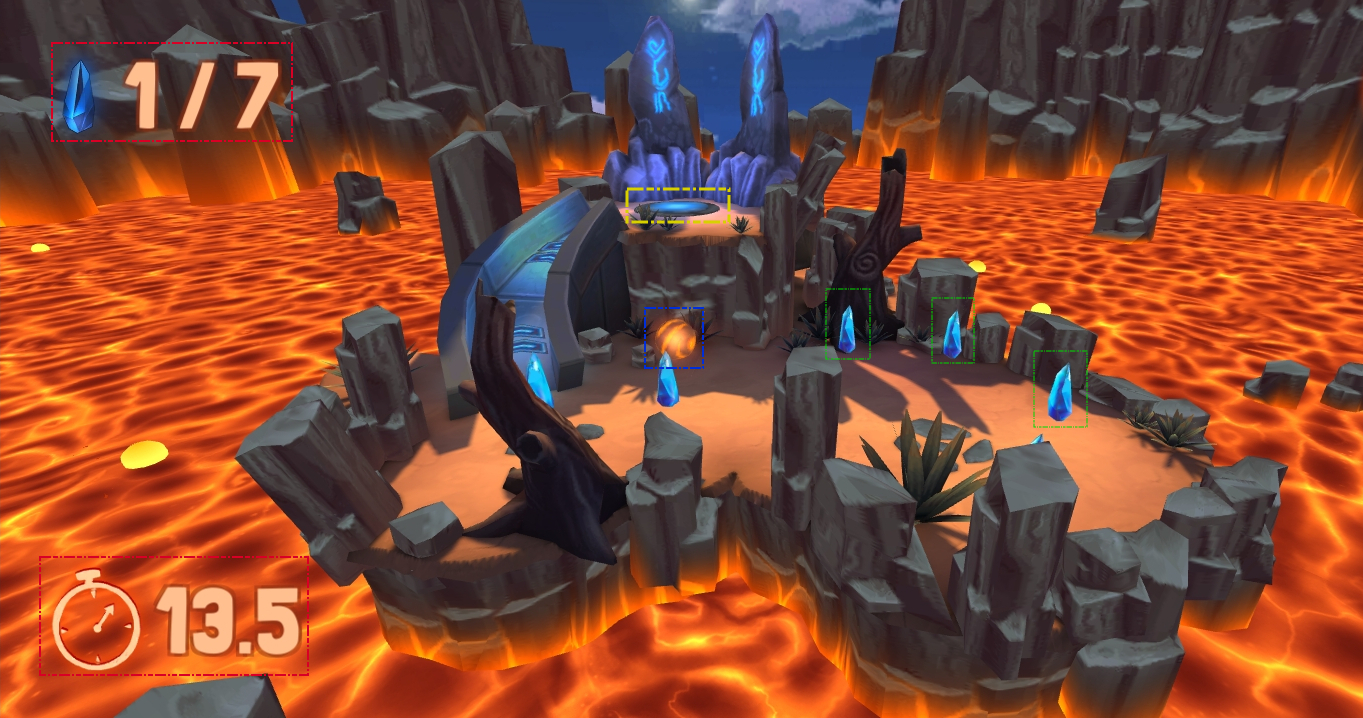
\includegraphics[scale=0.3]{img/balloma_scene.jpg} 
		\caption{Balloma's scene sample. Elements of scene are: a) The ball (blue), b) Floating elements (green), c) Score records (red), d) Target position (yellow)}
		\label{fig_scene}
	\end{figure}
   
   Each scene contains a constrained little terrain world with elements arranged and boundaries that if crossed makes the scene end. The scene's main element is a ball the player should control and carry to a remarked target position in the scene. To control such ball the player should touch and swipe the device's screen inputing a direction and speed he wants the ball to take. Once the ball is positioned at target, scene ends, a score is given to user and next scene is unlocked. 
   
   
   
   While the user carries the ball to target he can make the ball go trough floating elements in the scene which makes the score increase. Also a timer is included in the scene which influences the final score, lower scene's completion running times provides higher rewards.
   
   Figure \ref{fig_scene} presents the game's first scene which appears unlocked by default. In Figure \ref{fig_scene} the ball is bounded by a blue box. The blue diamonds bounded with a green box appears floating in the scene, if reached by the ball makes the score (upper left red box) increase. Target position is remarked inside a yellow box. Also there is a timer (lower left corner red box) that influences the final score.
   
   \section{Environment}
   
	An interface is implemented to provide a RL suitable environment by which the agent can interact with the game to construct the optimized policy. Since the game runs in Android, the environment should provide a controlling interface with an android physical or virtual device. Such functionality can be attained through the Android Debug Bridge (adb\footnote{https://developer.android.com/studio/command-line/adb}). 
	
	\subsection{States}	
	
	In this proposal the states are represented by raw scene frames of 240x240. It means at each time step $t$ the environment is at state $s_t \in \mathbb{R}^3$ formatted as a tensor of shape $(240, 240, 3)$. A similar approach was presented in \cite{ddpg_2015} and \cite{replay_buffer_2015}, however scenes in those works are 2D spaces and in this case it is 3D. Frames are cropped to exclude score indicators and focus on more important pixels.
	
	\subsection{Actions}
	
	On each time step the agent can chose to take an action $a_t \in \mathbb{R}^3$. Actions are presented as a tuple $a_t=(\vartheta, \varkappa, \xi)$ that describes the swipe action: \textit{a)} $vartheta$ size of the vector drawn by the swipe, \textit{b)} $\varkappa$ angle with respect to screen horizontal of the vector drawn by the swipe and \textit{c)} $xi$ speed at which swipe is drawn.
	
	Each episode starts with the first swipe inputted by the agent. If the balls falls off the terrain world or get to target position, environment is set into a terminal state. Also it will be constrained in time to avoid long episodes. 
	
	\section{Reward function}
	
	At each time step, after the agent choses an action $a_t$ and such action is applied to environment, a reward $r_t$ is observed. If an episode gets into a failed terminal state (e.g ball falls out) reward of that step is computed as -1. On the other hand if episode ends successfully (i.e the ball hits the target), reward of that step is computed as +2.
	
	For others time steps, reward is computed taking into account two coefficients: \textit{a)} ratio between floating diamonds currently gathered over total ($\omega$) and \textit{b)} episode time passed since it started ($\varphi$). Also each parameter is multiplied by a weight coefficient $\alpha$ and $\beta$ that regulates its importance, it permits experimenting different parameter's level of impact. In such cases reward is computed as:
	
	\begin{equation}
	  r(s_t, a_t) = \alpha \frac{\omega_t}{\omega_N} - \beta \frac{\varphi_t}{\varphi_N} 
	\end{equation}
	
	
	There exists in the scene an object providing information on how many diamonds has been collected. During training, after an action is inputed into the scene a frame is captured and processed to extract the information needed to compute reward. In order to extract that data, which is used by the reward function, in this work was implemented a picture matching procedure in which crops of predetermined portions of the scene are compared with previously tagged crops of the digits as it is rendered in the scene. 

	For each digit from 0 to 9, crops were previously gathered and tagged. Such digit images are compared with the pixels cropped from scene at specific coordinates it is expected the element with current scoring appears, in order to determine diamonds gathered at each step, during training. 
	
	Before comparison, crop's color space is transformed into binary. Then the \textit{height}X\textit{weight} shaped crops are subtracted and bits in the result are summed. If the result is below a predefined threshold, the crop is classified with the digit of the crop it was matched against.
	  
	Since it is necessary before hand the exact position of the elements in screen, this approach is dependent on the device's screen size, thus should be manually adjusted for each device it is used on. The code accompanying this report contains coordinates and crops compatible with a Samsung S8+ device screen. This method worked properly in 100\% of cases.
	
	  \section{Benchmark Model}
	  
	  Previous researches have addressed video game playing agents with reinforcement learning. Mnih et al.  \cite{replay_buffer_2015} created Atari video game playing robots trough the use of an adaptation to Deep Q-Learning. This approach is considered as Deep Reinforcement Learning since makes use of neuronal networks to map states to Q-values directly. The method was tested on 49 Atari games assessing reward evolution throughout training. It was achieved professional human players comparable performance. 
	  
	  Deep Deterministic Policy Gradients \cite{ddpg_2015}, the method presented in this work, was used by its authors to create an agent that plays Torc, a racing video game. They compared effectiveness of the method when applied on low-dimensional features like acceleration, braking and steering and with high-order features like pixel representations (i.e game raw frames), assessing reward evolution throughout training. It was demonstrated by experimentation that similar performance is attained for both features presentations.

	In this work both approaches has been implemented and applied to Balloma Video Game playing agent. More details are presented in coming sections.
	  
	  \section{Results}
	  
	  \begin{figure}[t]
\centering
\begin{minipage}{0.45\textwidth}
	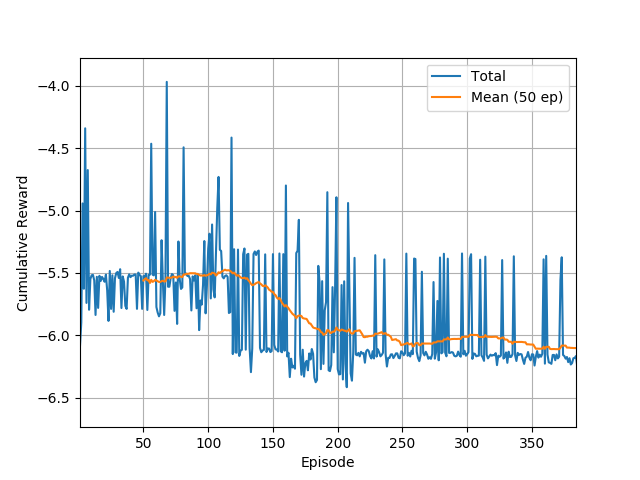
\includegraphics[scale=0.55]{img/cumulative_reward.png}
	\caption{Cumulative Reward evolution through episodes on DDPG approach.}
	\label{fig:reward}

	\end{minipage}
	\hspace{0.2cm}
	\begin{minipage}{0.45\textwidth}
		\centering
		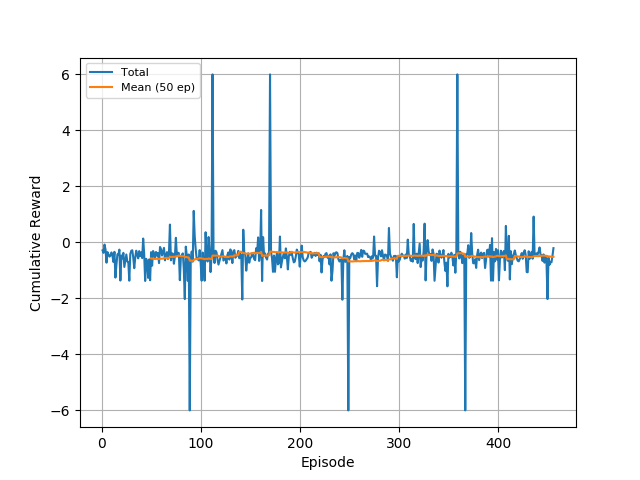
\includegraphics[scale=0.55]{img/rewardDQN.png}
		\caption{Cumulative Reward evolution through episodes on Deep Q-Learning approach.}
		\label{fig:reward_1}
		\centering
	\end{minipage}	
	\end{figure} 
	  
	  It was implemented two Reinforcement Learning setups composed by an agent, represented by a Convolutional Neuronal Network (ConvNet) and an environment, representative of Balloma Video Game, driven by an iterative procedure in which at every step the agent interacts with the environment and information from that interaction is used to adjust the agent's behavior with the goal of incrementing the reward the agent obtains when interacting with the environment. 
	  
	 The first setup follows the Actor-Critic Deep Deterministic Policy Gradient, approach in which game actions are inferred by a ConvNet adjusted from experiences obtained by interaction with Balloma Video Game. Each experience is compound of an action, reward and game scene frame, obtained by inputting the inferred action into the video game running in an android device and capturing the rendered frame. Another Neuronal Network, called the Critic, evaluates how well the Actor is performing and outputs a gradient that is used to adjust the Actor towards minimizing the loss and increasing the reward obtained from environment.
	 
	 For each model there are a local and a target model, the former is updated on each training iteration in a approximation with a supervised learning using the target as the ground truth. On each model fit the target is soft-updated by increasing its weights based on the local model rather then exactly copying it.
	 
	 It was also implemented a Deep Q Network \cite{deep_q_n} that represents the Q-Value function and maps states to Q-Values. Such network follows the same architecture as the Actor ConvNet as presented in Table \ref{tab:actor_arch}. Since this approach is not compatible with continuous valued actions two changes are applied with respect to DDPG implementation, in order to make it compatible: \textit{a)} vector size and swipe speed are fixed (i.e not inferred by the network), \textit{b)} only angle is inferred by the DQN. It was considered that angle was action's most prominent feature.  
	 
	 \subsection{Actor ConvNet}
	 
	 The Actor Convolutional Neuronal Network architecture is presented in Table \ref{tab:actor_arch}. A similar architecture was proposed in the original paper of Deep Deterministic Policy Gradient \cite{ddpg_2015}. 
	 
	 \begin{table}[h] 
	\centering
%	\begin{tabular}{p{2cm} p{0.5cm} p{1.3cm}} 
	\begin{tabular}{l l l} 
		\toprule 
%		& & \multicolumn{2}{c}{Metric} \\ 
%		\cmidrule(l){3-4} 
		Layer (type) & Output Shape & Param \# \\ 		
		\midrule
		$states (InputLayer)$ & (None, 84, 296, 9) & 0\\ 
		$conv2d\_1 (Conv2D)$ & (None, 83, 295, 32) & 1184  \\ 
		$conv2d\_2 (Conv2D)$ & (None, 82, 294, 32) & 4128  \\
		$conv2d\_3 (Conv2D)$ & (None, 81, 293, 32) & 4128  \\
		$dense\_1 (Dense)$  & (None, 81, 293, 200) & 6600  \\   
		$dense\_2 (Dense)$ & (None, 81, 293, 200)  & 40200 \\
		$raw\_actions (Dense)$ & (None, 81, 293, 3) & 603  \\
		$global\_average\_pooling2d\_1$ & (None, 3) & 0  \\
		$actions (Lambda)$ & (None, 3) &  0 \\
		\midrule 
		\midrule
		Total params: 56,843 & &  \\
		Trainable params: 56,843 & &  \\
		Non-trainable params: 0 & & \\

		\bottomrule 
	\end{tabular}
	\smallskip 
	\caption{Agent's Actor and Deep Q Network ConvNet Architecture.} 
	\label{tab:actor_arch} 
\end{table}

The Actor's ConvNet architecture consists of 3 Conv layers of 32 filters each, without pooling layers. It is followed by two fully connected layers with 200 units. It was used Adam \cite{adam_2014} for learning the network parameters with a learning rate of $10^{-4}$. It is used the rectified non-linearity \cite{relu_2011} for all layers. The final output layer of the actor is a $tanh$ layer, to bound the actions. The final layer weights and biases are initialized from a uniform distribution $[3 * 10^{-4}, 3 * 10^{-4}]$, to ensure the initial outputs for the policy are near zero.
	 
	 \subsection{Critic Neuronal Network}
	 
	 The Critic's Neuronal Network architecture is presented in Table \ref{tab:critic_arch}. A similar architecture was proposed in the original paper of Deep Deterministic Policy Gradient \cite{ddpg_2015}. 
	 
	 
	 
	  \begin{table}[h] 
	\centering
	\begin{tabular}{l l l l} 
		\toprule 				
		Layer (type)          &          Output Shape   &      Param \#   &  Connected to  \\
		\midrule           
		$states (InputLayer) $   &         (None, 84, 296, 9)  & 0 &    \\                          
		$flatten\_1 (Flatten) $   &         (None, 223776) &      0 &          $states[0][0]   $    \\
		$actions (InputLayer)$  &  (None, 3)    &        0      &             \\
		$dense\_1 (Dense)  $ &  (None, 32)  & 7160864  &   $flatten\_1[0][0] $ \\
        $dense\_3 (Dense)  $ & (None, 32) & 128 &  $actions[0][0]$ \\
		$dense\_2 (Dense) $  & (None, 64) & 2112  &  $dense\_1[0][0] $ \\ 
        $dense\_4 (Dense) $ & (None, 64) & 2112 &  $dense\_3[0][0]$ \\
		$add\_1 (Add) $ & (None, 64) &  0  & $dense\_2[0][0] $ \\                   
                                                                &&& $dense\_4[0][0] $ \\
		$activation\_1 (Activation) $ & (None, 64) & 0 & $add\_1[0][0]$ \\
		$q\_values (Dense) $ & (None, 1)& 65 & $activation\_1[0][0] $ \\
		\midrule
		\midrule
Total params: 7,165,281 & & &\\
Trainable params: 7,165,281 & & & \\
Non-trainable params: 0 & & & \\

		\midrule 
		\bottomrule 
	\end{tabular}
	\smallskip 
	\caption{Agent's Critic Neuronal Net Architecture.} 
	\label{tab:critic_arch} 
\end{table}
	 
	 The Critic's network architecture consists of two inputs for states and actions respectively. Since states are tensors, that input is flattened before hidden layers. Following there are three dense layers in a row with 32, 32 and 64 units respectively.
	 
	 It was used Adam \cite{adam_2014} for learning the network parameters with a learning rate of $10^{-4}$. It is used the rectified non-linearity \cite{relu_2011} for all layers. The final layer weights and biases are initialized from a uniform distribution $[3 * 10^{-3}, 3 * 10^{-3}]$, to ensure the initial outputs for the policy are near zero.
	 
	 \subsection{Training}


	 \begin{figure}[t]
\centering
\begin{minipage}{0.4\textwidth}
	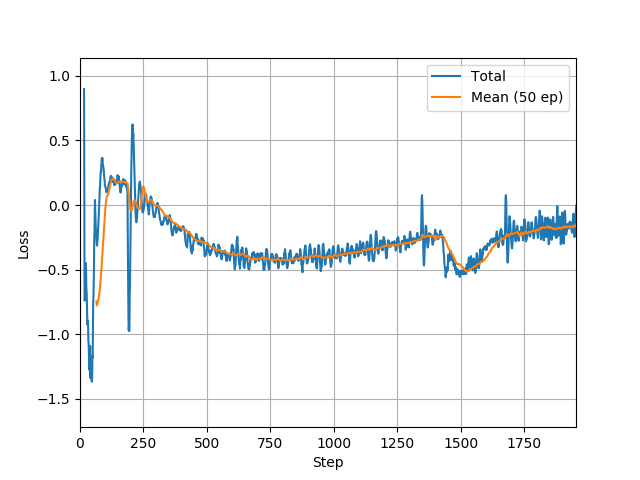
\includegraphics[scale=0.5]{img/loss.png}
	\caption{Action gradient loss evolution through subsequent steps on DDPG approach.}
	\label{fig:loss}

	\end{minipage}
	\hspace{0.5cm}
	\begin{minipage}{0.4\textwidth}
		\centering
		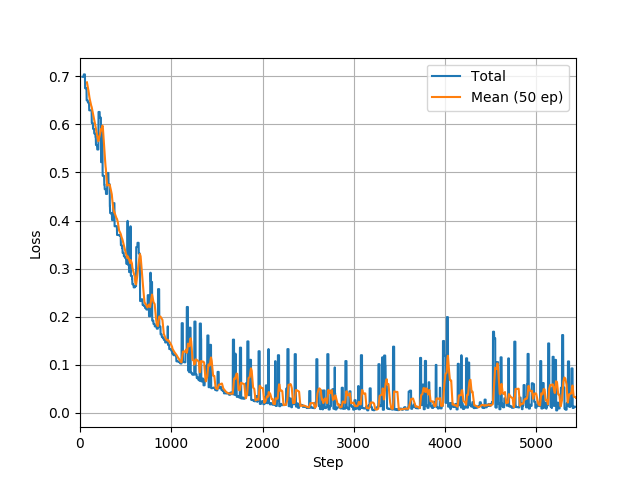
\includegraphics[scale=0.5]{img/lossDQN.png}
		\caption{Q-Value loss evolution through subsequent steps on Deep Q-Learning approach.}
		\label{fig:loss_1}
		\centering
	\end{minipage}	
	\end{figure}
	 
%	  \begin{figure}[!h]
%		\centering
%		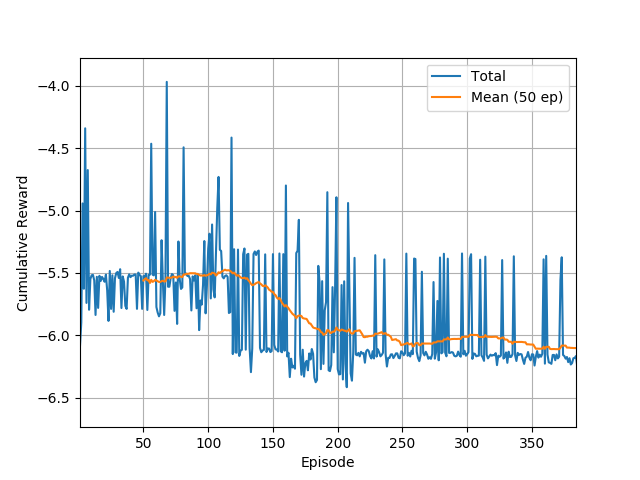
\includegraphics[width=0.9\columnwidth]{img/cumulative_reward.png} 
%		\caption{Cumulative Reward evolution through episodes.}
%		\label{fig:reward}
%	\end{figure}
	
	 In order to fit the Actor and Critic models it was executed an iterative process in which each iteration is called as episode. At each episode the Actor's model is used to select actions that are applied to video game running in an android device, through \textit{adb}. Some random noise is added to such action in order to provide exploration.
	 
	 For DQN actions are selected following a Greedy in the Limit with Infinite Exploration approach. A coefficient epsilon controls exploration-explotations probabilities, used to decide when to select a random action or the action that maximizes reward, based on the Q-Network prediction. At each step, epsilon is decreased with a decay rate of 0.001.
	 
	 \begin{figure}[!h]
		\centering
		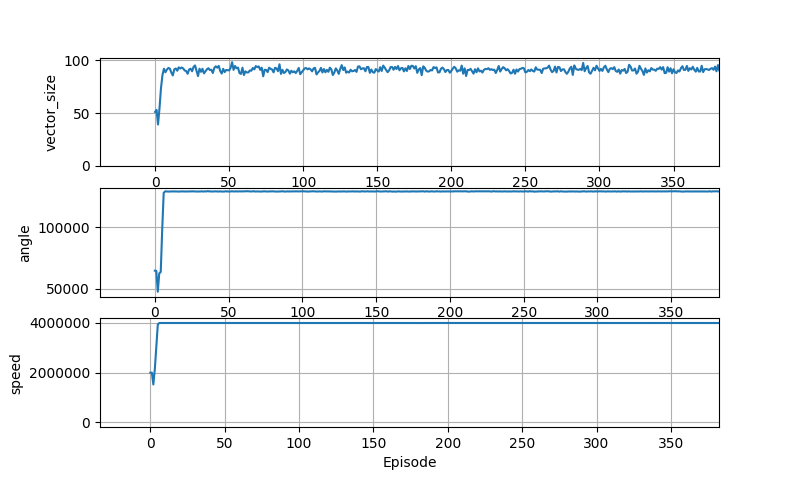
\includegraphics[width=0.9\columnwidth]{img/action.png} 
		\caption{Action parameter's values evolution throughout training on DDPG approach.}
		\label{fig:actiosDDPG}
	\end{figure}
	 
	 On each step of an episode, an experience is gathered containing: \textit{a)} the state before action is performed, \textit{b)} the action itself, \textit{c)} the reward returned by environment after applying such action and \textit{d)} the state after the action was executed. Such experiences are stored in a replay buffer \cite{rep_buffer}.
	 
	 
	 \begin{figure}
		\centering
		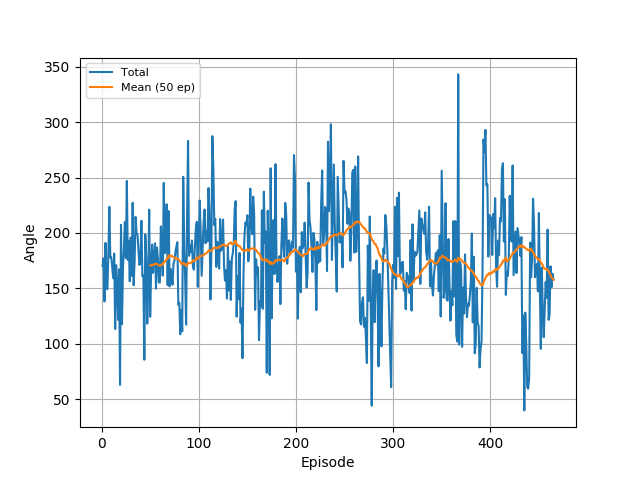
\includegraphics[scale=0.8]{img/angleDQN.png} 
		\caption{Action's angle parameter values evolution throughout training on Deep Q-Learning approach.}
		\label{fig:angledqn}
	\end{figure}
	 
	  At the end of each episode, if the replay buffer contains at least 16 experiences a new model fit iteration is executed. A batch of 16 experiences are randomly selected from buffer and inputted into the Critic model in order to obtain action gradients in the DDPG approach. Such gradients are used to compute the loss and fit the Actor model.
	  	  
	For each episode, it is computed a cumulative reward as the sum of each step reward. Figure \ref{fig:reward} presents evolution of cumulative reward throughout training and the mean for 50 episodes, for the DDPG setup. The trends indicates a rather random or erratic behavior, in which reward is not enhanced between subsequent episodes, tendency is to lower rewards as more episodes passed. On the other hand, as seen in Figure \ref{fig:reward_1}, for the Deep Q-Learning approach higher reward scores were attained, some even positive which does not happens for DDPG. Also reward's trend for DQN is to stability or increase rather than decline.
	
	
	
	Figure \ref{fig:loss} presents evolution of Actor's model loss throughout training, for each step, on the DDPG approach. Since model's weights are not reseted at every step or new episode it is expected that loss will tend to decrease. However it gravitates around zero, decreasing and increasing almost evenly.
	
	Figure \ref{fig:loss_1} presents evolution of agent's model loss throughout training, for each step, on the Deep Q-Learning approach. Different than with DDPG in this case it is more evident a pattern towards decline as further episodes are experienced.
	
	
	Figure \ref{fig:loss} presents the evolution of the parameter's values that compounds actions on the DDPQ approach. Here the trends are to increment and stabilization. This behavior might be caused by the distribution of the exploration noise applied, it should be studied if the noise strategy selected is adequate for the setup in this work.
	
	Figure \ref{fig:angledqn} shows mean angle values for episode. Here exploration is benefited over exploitation which is recommended since reward stills does not presents a steady growth at the moment graphs were plotted. Although exploration is favored, it eventually starts to be spotted a pattern, which can be interpreted as the agent learning a sequence of actions.
	
	\section{Conclusions}
	
	This work presented two Reinforcement Learning setups, projected, implemented and executed, following the Deep Deterministic Policy Gradients \cite{ddpg_2015} and Deep Q-Learning approaches \cite{replay_buffer_2015}. Such setups was used to train an agent to play Balloma video game. 
	
	As experimentation demonstrated, Deep Q-Learning presented better results than DDPG. Cumulative reward evolution throughout training presented a trend towards decrease in subsequent episodes for DDPG however for DQN episode's mean reward throughout training tends to stability and growth rather than decrease. Loss did not decreased as expected throughout training for DDPG and decreased steadily for DQN. Also, for DDPG, action parameter's values trends to exploitation with no significant return in reward increase, in which case exploration would have been the expected behavior, nevertheless for DQN a pattern starts to appear towards more recent episodes which can be interpreted as the agent learning a sequence of actions.
	
	It is worth noting that the approach this work follows was previously used in a similar setup, in which an agent was trained to play video games. However, different than in this work, previous experiences was applied to a 2D world game and in this case it is being applied to a 3D world game.
	
	In future works, further experimentation should be performed. New models architectures can be experimented with dropout, normalization, pooling and different weight initialization strategies, to avoid actions stagnation and favor exploration. Also new noise modifying strategies can be explored.
 

\begin{thebibliography}{1}
% Here are a few examples of different citations 
% Book

\bibitem{ddpg_2015}
  Lillicrap, Timothy P., et al. "Continuous control with deep reinforcement learning." arXiv preprint arXiv:1509.02971 (2015).
  
  \bibitem {actor_critic_2000} 
  Konda, Vijay R., and John N. Tsitsiklis. "Actor-critic algorithms." Advances in neural information processing systems. 2000.
  
\bibitem{silver_2004}
  David~Silver, Guy~Lever, Nicolas~Heess, Thomas~Degris, Daan~Wierstra, and Martin~Riedmiller. 2014. Deterministic policy gradient algorithms. In Proceedings of the 31st International Conference on International Conference on Machine Learning - Volume 32 (ICML'14), Eric P. Xing and Tony Jebara (Eds.), Vol. 32. JMLR.org I-387-I-395.
  
  \bibitem{replay_buffer_2015}
  
  Mnih, Volodymyr, Kavukcuoglu, Koray, Silver, David, Rusu, Andrei A, Veness, Joel, Bellemare,
Marc G, Graves, Alex, Riedmiller, Martin, Fidjeland, Andreas K, Ostrovski, Georg, et al. Humanlevel control through deep reinforcement learning. Nature, 518(7540):529–533, 2015.

\bibitem{bellman_equation}

(2011) Bellman Equation. In: Sammut C., Webb G.I. (eds) Encyclopedia of Machine Learning. Springer, Boston, MA

\bibitem{mnist}

	LeCun, Y. \& Cortes, C. (2010), 'MNIST handwritten digit database'.
	
\bibitem{adam_2014}
	Kingma, D. P., and J. L. Ba. "Adam: A method for stochastic optimization. arXiv 2014." arXiv preprint arXiv:1412.6980 (2014).
	
\bibitem{relu_2011}
	Glorot, Xavier, Bordes, Antoine, and Bengio, Yoshua. Deep sparse rectifier networks. In Proceedings of the 14th International Conference on Artificial Intelligence and Statistics. JMLR W\& CP Volume, volume 15, pp. 315–323, 2011.
	
	\bibitem{rep_buffer} 
	
	Wawrzynski, Paweł and Tanwani, Ajay Kumar. Autonomous reinforcement learning with experience replay. Neural Networks, 41:156–167, 2013.
	
	\bibitem{deep_q_n}
	Mnih, Volodymyr, Kavukcuoglu, Koray, Silver, David, Graves, Alex, Antonoglou, Ioannis, Wierstra, Daan, and Riedmiller, Martin. Playing atari with deep reinforcement learning. arXiv preprint arXiv:1312.5602, 2013.
	 
\end{thebibliography}

% This is a hand-made bibliography. If you want to use a BibTeX file, you're on your own ;-)














\end{document}


